% CS 229 Project Paper
% This is for the milestone; though we're expanding it for the final draft,
% it will probably be useful to have around afterwards.

% Goal: fill three pages with useful background data, plans, stuff.

\documentclass{amsart}
% At this point, my macros file is a bit disorganized. But it ought to be
% usable.

% For page margins
\usepackage[margin=1in]{geometry}
\usepackage{xcolor}
\usepackage{graphicx}
\usepackage{mathtools}
\usepackage{enumerate}
% Sets font to Garamond. Feel free to change this or remove it.
% \usepackage[garamond]{mathdesign}
\usepackage{hyperref}
% Makes figure labels work better
\usepackage[all]{hypcap}

% Note: we might want to use fancyhdr. We can worry about that later.
\pagestyle{plain}

\newcommand{\N}{\mathbb N}
\newcommand{\Z}{\mathbb Z}
\newcommand{\Q}{\mathbb Q}
\newcommand{\R}{\mathbb R}
\newcommand{\T}{^{\mathrm T}\!}
\newcommand{\ud}{\,\mathrm d}
\newcommand{\dfr}[2]{\frac{\mathrm d #1}{\mathrm d #2}}
\newcommand{\pfr}[2]{\frac{\partial #1}{\partial #2}}
\DeclareMathOperator*{\argmax}{arg\,max}
\DeclareMathOperator*{\argmin}{arg\,min}

% I like bold vectors, and this allows bold Greek letters too.
% Feel free to change or remove this.
\renewcommand{\vec}[1]{\boldsymbol{\mathbf{#1}}}

% So that we have \paren{...} instead of \left( and \right)
\DeclarePairedDelimiter\paren{(}{)}
\DeclarePairedDelimiter\ang{\langle}{\rangle}
\DeclarePairedDelimiter\abs{\lvert}{\rvert}
\DeclarePairedDelimiter\norm{\lVert}{\rVert}
% Swap paren* and paren, etc., so that the normal version resizes by default.
% Meanwhile, one can use \paren*[\Big]{...} to customize the size easily.
% It would be interesting to wrap this up into a custom \definedelimiter command...
\makeatletter
    \let\oldparen\paren
    \def\paren{\@ifstar{\oldparen}{\oldparen*}}
    \let\oldang\ang
    \def\ang{\@ifstar{\oldang}{\oldang*}}
    \let\oldabs\abs
    \def\abs{\@ifstar{\oldabs}{\oldabs*}}
    \let\oldnorm\norm
    \def\norm{\@ifstar{\oldnorm}{\oldnorm*}}
\makeatother

% This allows x"i -> x^{(i)} and x"{i+1} -> x^{(i+1)}
\catcode`\"=13
\newcommand{"}[1]{^{(#1)}}

\newcommand{\e}{\varepsilon}
\newcommand{\E}[1]{\cdot 10^{#1}}

\geometry{margin=0.8in}
\begin{document}
\title{Astronomical Implications of Machine Learning}
\author{
	\lowercase{\href{mailto:adebray@stanford.edu?subject=CS\%20229\%20Project}}{Arun Debray}\\
	\lowercase{\href{mailto:wur911@stanford.edu?subject=CS\%20229\%20Project}}{Raymond Wu}\\
	\today
}
\maketitle

% Do we need a table of contents? Probably not.
%\tableofcontents

% I started writing things. You are welcome to edit them!

% Abstract might not be necessary
\begin{abstract}
In this project we aim to use supervised learning to develop a classifier for stellar lightcurves
 to detect whether they demonstrate the existence of exosolar planets. We will use various features selection methods;
 in particular we will be using dynamic time warping to measure the similarity between two temporal sequences.
\end{abstract}
\section{Introduction}
% What are exoplanets? How are they detected?
The recent discoveries of planets around stars other than our own is among the most significant trends in astronomy today. Long debated by philosophers and physicists alike, no such planets were known until 1992, when two planets were discovered around a star called PSR B1257+12. In the two decades since then, over a thousand such planets have been discovered, diverse in many ways. Thanks to these discoveries, astronomers are learning more about planetary systems other than our own, responding to these questions about other solar systems and even how probable Earth-like life could be in the universe.

In this paper, we will use the following standard terminology.
\begin{itemize}
	\item An \emph{exosolar planet} is defined as in \cite{Ovr} to be a planet that orbits a star other than the Sun.\footnote{The words \emph{exoplanet}, \emph{exosolar planet}, and \emph{extrasolar planet} all mean the same thing, and are used interchangeably.} The standard definition of a planet has two kinds of ambiguity: very low-mass objects in our solar system, such as Pluto, were defined to be ``dwarf planets,'' and the boundaries of this definition aren't entirely clear. Very high-mass planets, however, resemble very small stars; though they don't undergo hydrogen fusion, they look very much like a dim type of star called a brown dwarf. The boundary is somewhat arbitrarily delineated at 13 Jupiter masses. However, neither of these is a great concern in this paper: science is yet unable to detect Pluto-sized worlds around another star, so the low-mass ambiguity does not arise in this data, and the high-mass boundary is not as important: a classifier that discovers planets and small brown dwarfs is still useful. However, it will be helpful to distinguish these systems from eclipsing binaries (see below).
	\item \emph{Planetary transit} is a method of exoplanet detection, In general, because planets are very dim relative to their bright host stars, they cannot be directly imaged, in the same way that it is difficult to detect a firefly near a searchlight from afar. Thus, several indirect methods exist. Planetary transit repeatedly checks the brightness of a star over time; periodic, regular dips in this output sometimes happen because an exoplanet crosses between its sun and the observer. Thus, a planet may be detected without direct observation. See \cite{Trs} for more information on transiting exoplanets.
	\item A \emph{lightcurve} is a graph of a star's brightness over time. A transiting exoplanet will thus manifest itself as a lightcurve that is relatively constant, but with regular, small dips corresponding to the transits. See Figure~\ref{curves} for two examples.
	 The brightness is often given in units of magnitude rather than strict luminosity, because the logarithmic magnitude scale is generally easier to work with.
	\begin{figure}
	\centering
	\label{curves}
	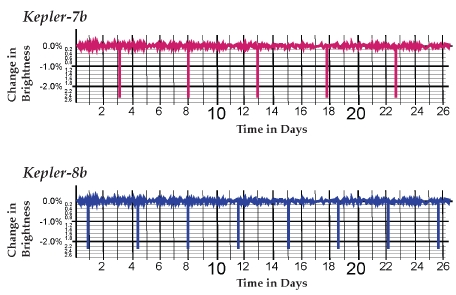
\includegraphics[width=6in]{transit_lightcurve}
	\caption{Lightcurves (graphs of stellar brightness versus time) of two planetary transit systems discovered by Kepler. The regular small dips correspond to the planet passing in front of its sun and slightly diminishing the observed magnitude. Source: NASA}%http://kepler.nasa.gov/education/activities/transitTracks/ if we make a real bibliography
	\end{figure}
	\item An \emph{eclipsing binary} is a pair of stars that orbit each other, but such that each eclipses the other from the Earth's point of view during the orbit. These generally don't contain transiting exoplanets, but instead form an important negative example. Their lightcurves look like those of exoplanets, but they aren't exoplanets.
\end{itemize}
% Why Kepler?

Until recently, most exoplanets weren't detected by transit; astronomers used any of several other methods to find them. However, when the Kepler telescope was launched, it provided a wealth of data about transiting exoplanets, in particular showing that many stars could be surveyed at once. Since Kepler provided such a wealth of data about exoplanets, we decided to try to train a classifier on its lightcurves.%expand? TODO
% Planet Hunters, maybe

\section{Methodology}
We obtained Kepler light curves from the Mikulski Archive for Space Telescopes (see \cite{mast}). Lightcurves are stored in the \texttt{.fits} file format, so we used the AstroPy Python library, found at \cite{AstroPy}, to parse them. We first divided light curves into those corresponding to exoplanets and those corresponding to non-exoplanets. The non-exoplanets contained \"non-variable\" stars, which had relatively uniform light curves as well as stars with variable light curves that did not have exoplanets. These variable light curves were caused by other reasons, including binary star systems and intrinsically variable stars. The light curves are represented as time series data, which means that each light curve is represented by a series of attributes at each time point within some range. The attributes of the light curve stored in the binary table include:
\begin{itemize}
	\item TIME: The time at the midpoint of the light curve
	\item SAP\_FLUX: Simple aperture photometry flux in units of electrons per second contained in the optimal aperture pixels
	\item SAP\_FLUX\_ERR: The error in SAP flux in electrons per second
	\item SAP\_BKG: The total background flux summed over the optimal aperture
	\item SAP\_BKG\_ERR: The error in the background flux
	\item PDCSAP\_FLUX: Flux after Presearch Data Conditioning (PDC) has accounted for systematic error sources such as drift or focus change
	\item PDCSAP\_FLUX\_ERR: The error in PDCSAP flux
	\item PSF\_CENTR1: The column centroid obtained by fitting the point spread function
	\item PSF\_CENTR1\_ERR: The error in PSF centroid 1
	\item PSF\_CENTR2: The row centroid obtained by fitting the point spread function
	\item PSF\_CENTR2\_ERR: The error in PSF centroid 2
	\item MOM\_CENTR1: The column value for the flux weighted centroid (first moment)
	\item MOM\_CENTR1\_ERR: The error in MOM centroid 1
	\item MOM\_CENTR2: The row value for the flux weighted centroid (first moment)
	\item MOM\_CENTR2\_ERR: The error in MOM centroid 2
	\item POS\_CORR1: The column position correction based on bright stars 
	\item POS\_CORR2: The row position correction based on bright stars
\end{itemize}

We decided early on that we should build a classification model on features extracted only from a couple of these attributes since not all the attributes were relevant to our query. We decided to go with attributes "SAP\_FLUX", "SAP\_BKG", "PDCSAP\_FLUX", "MOM\_CENTR1", "MOM\_CENTR2", "POS\_CORR1", "POS\_CORR2". These values in particular were nonnull and relayed important data about the light curve. 

Since our lightcurves are time series, which are large series of data points separated by a uniform time interval, it is both extremely difficult and unhelpful to train any sort of classifier over the raw data points. Instead, we will need to extract features from each time series. These features have to be both manageable and descriptive of the light curve.

%These lightcurves can be thought of as feature vectors in an enormously large-dimensional space, since they correspond to several data points over a large number of distinct observations. Thus, it will be necessary to do some feature selection.

%For this milestone, we chose to explicitly work with a few simple features rather than running a larger feature-selection algorithm. Specifically, for each data point above, we calculated the mean and standard deviation of the element over the entire time series. 
%From here we can attempt to do several things. We can try to run some supervised learning classifiers using the arithmetic mean, maximum value, minimum value, range, and standard deviation of each data attribute as opposed to treating it as a time series. 
%This primitive form of filtering a time series into its global features is a crude way of using the time series data, but for now it should gives us a rough idea of how our data can be used for classification. We can then use some of the classifiers we learned, such as logistic regression, Na\"ive Bayes classifiers, or support vector machines to train a classifier on these new features. 
We decided to try a variety of feature selection methods. Initially, we decided to look for global features such as the arithmetic average, maximum, and minimum values for each attribute. These global features provide very high-level, general descriptions of the time series. Thus they provide a good set of initial features, but can only provide a limited amount of detail. Using metafeatures can be used to provide a more accurate description of the time series, but we decided to opt for a different type of feature.

Given that we were examining light curves, which vary in time and speed due to differences in the size and shape of the orbiting planets as well, differences in orbital periods, and differences in the instrument recordings, we want to be able to detect common patterns that are indicative of exoplanets regardless of these differences between different planets and stars. So to do this, we turned to an algorithm called dynamic time warping. Dynamic time warping (DTW) calculates the optimal match between two time series by calculating a measure of similarity independent of the time, speed, and acceleration of the time series. 

We decided to use dynamic time warping to calculate the similarity of each light curve with a "baseline" light curve. To find an appropriate "baseline" light curve, we took a relatively flat light curve from our training set of light curves without exoplanets. Then we used dynamic time warping to calculate a measure of similarity between each light curve and this "baseline". We used this result as one of our features in addition to our global features.

After extracting all of our appropriate features, we needed to train a classifier. We used an open source machine learning algorithm suite called Weka, developed at the University of Waikato in New Zealand. We used a variety of classification methods including logistic regression, Na\"ive Bayes, support vector regression (SVR), and multilayer perceptron. We found that SVM did not work particularly well, so we used a modified SVM algorithm called RegSMOImproved\cite{SMOreg}. In particular, we used a polynomial kernel to map the data to a higher dimension and then use the altered SMO algorithm to calculate a regression model. We also made use of the multilayer perceptron, an artificial neural network model that learns through backpropgation. 

We trained our classifiers on our data sets using 10-fold cross validation.
%We are currently using an optimal margin classifier with the linear kernel induced by $\phi(\vec x) = \vec x$. We specifically use the \textsc{Liblinear} classifier \cite{LibLinear} to accomplish this. However, given the relative complexity of the problem, we do not expect this to ultimately be the best approach. We chose it in order to begin classifying data, so that we have actual numbers to work with, rather than just ideas. 

%Given that our data is in the form of time series, we will want to look at different forms of time series analysis, such as dynamic time warping or Hidden Markov Models. The Weka library, found at \cite{Weka}, provides implementations of such algorithms. This, combined with a more powerful feature-selection algorithm, should give us a more effective classifier.


\section{Results}
We had 150 light curves that were either confirmed exoplanets or were labeled as exoplanets but unconfirmed as of August 2013. We had 103 light curves that were confirmed to not be exoplanets. So in total our training set size was 253 instances. 

% TODO Logistic Regression: model, correctly classified, incorrectly classified, mean absolute error, root mean squared error, confusion matrix

% TODO Naive Bayes

% TODO SMOreg

% TODO Multilayer perceptron

We can take a look at how our logistic regression model and multilayer perceptron model compare. The multilayer perceptron model takes all the input values (the fatures we collected) and returns a single value between -1 and 1 that is used to distinguish light curves with exoplanets (those with value greater than 0) and light curves without exoplanets (those with value less than 0). We can look at what values our models gave for our training set. The results are plotted in the curves below.
	\begin{figure}
	\centering
	\label{logistic}
	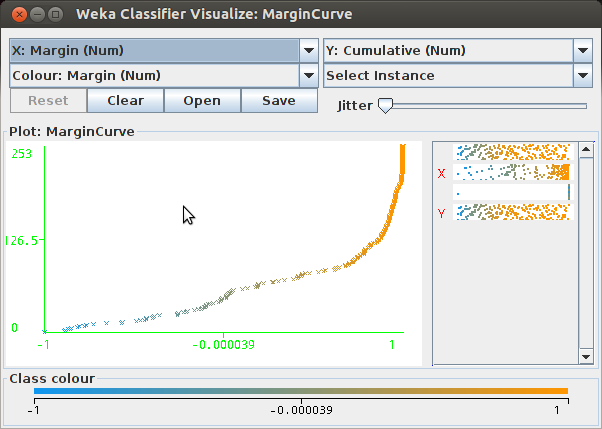
\includegraphics[width=6in]{logistic_regression}
	\caption{The predicted values for each light curve under the logistic regression model.}
	\end{figure}
	\begin{figure}
	\centering
	\label{multilayer}
	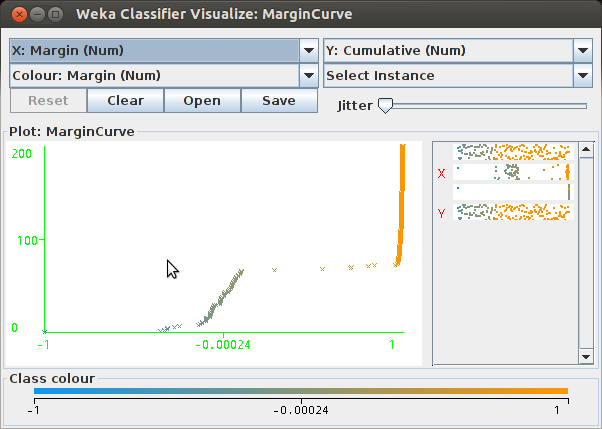
\includegraphics[width=6in]{multilayer_perceptron}
	\caption{The predicted values for each light curve under the multilayer perceptron model.}
	\end{figure}
	

\section{Analysis}
%One major problem so far is that we are lacking sufficient training and test instances. With a greater number of training instances, we can hopefully train a more accurate model that will be better at predicting labels for the test data instances. In particular, we are lacking a good number of data instances of confirmed exoplanets. In such a case, we would aim to use cross validation in order to conserve our data since we have so little. Thus we aim to not only find a larger data set, but also consider cross validation as a remedy to our lack of data.

% TODO talk about data

In particular, there are good reasons to assume that the problem is not necessarily linearly separable: intuitively, there are two major astronomical constraints on a lightcurve. If there are no dips in the lightcurve, then there is probably no transiting or eclipsing body around the parent star (or it is too small to be detected with current technology); yet if the changes in the magnitude are too large, then the transiting object is unlikely to be a planet; instead, it could be a brown dwarf or even a stellar companion (in which case the system is an eclipsing binary). Thus, the exoplanets lie in between these two constraints in the ``direction'' of the depth of the magnitude loss (i.e. some line in the feature space that accounts for these particular differences in the lightcurves), so a linear classifier that doesn't use a higher-dimensional kernel will be inaccurate.


\section{Future Work}
There are still several improvements that could be made. For one, we can run a clustering algorithm beforehand to group together light curves that have similar brightness and similar metafeatures. Thus, we would have clusters of stars that have similar apparent brightness. Then we can select from each cluster a light curve that contains a star that is known to not have any noticeable variability (exoplanet, binary system, variable star, etc). Then we can run the DTW algorithm to compare each star in that cluster to the non-variable star in order to obtain a even more "normalized" measure of similarity between light curves. 

Another improvement we could make is to try to use a multinomial classifier or a clusterer to be specifically classify the light curve as a binary star, a variable star, a transiting planet, or something else. Instead of just classifying to be able to tell whether there is a exoplanet or not, we could expand our attribute list and collect more features to generate a classifier that can provide more detailed classification. 

We could also train and test our classifiers on larger sets of data. As the Kepler project has been discontinued, we have a very limited training set to work with. Kepler has discovered over 3000 unconfirmed planet candidates, but only a little over 100 have been confirmed, which gives us a relatively small training set. And given that greater than expected noise and failure of Kepler's instrumentation has plagued the project, the data collected in the latter half of the project is likely dubious.  In the chance of another exoplanet-discovery project in the future, we will aim to continue training and testing our classifiers. But in the meantime, there are still hundreds of thousands of Kepler target light curves to be sorted through.
%As mentioned previously, we plan to look at more forms of time series analysis in order to obtain more information about our data. One thing we will consider in particular is dynamic time warping (DTW). Dynamic time warping is an algorithm for measuring the similarity between time sequences with varying time and speed. This will be helpful in confronting our problem because many exoplanets have different orbital periods or sizes, which makes comparing subtler features harder. Using DTW will allow us to compare the similarity of light curves that may have different periods, which will allow us to make a more general conclusion.

% bibliography of some sort
\begin{thebibliography}{9}
\bibitem{AstroPy}{
	Robiatille, Thomas P., et. al.
	\href{http://www.aanda.org/articles/aa/pdf/2013/10/aa22068-13.pdf}{\textit{Astropy: A community Python package for astronomy}}.
	Astronomy and Astrophysics, Volume 558, October 2013.
}
\bibitem{LibLinear}{
	R.-E. Fan, K.-W. Chang, C.-J. Hsieh, X.-R. Wang, and C.-J. Lin.
	\href{http://www.csie.ntu.edu.tw/~cjlin/papers/liblinear.pdf}{\textit{LIBLINEAR: A library for large linear classification}}.
	\href{jmlr.org}{Journal of Machine Learning Research} 9(2008), 1871-1874.
}
\bibitem{Weka}{
	Mark Hall, Eibe Frank, Geoffrey Holmes, Bernhard Pfahringer, Peter Reutemann, Ian H. Witten (2009);
	\href{http://www.sigkdd.org/sites/default/files/issues/11-1-2009-07/p2V11n1.pdf}{\textit{The WEKA Data Mining Software: An Update}};
	SIGKDD Explorations, Volume 11, Issue 1. 
}
% for the general overview, I guess?
\bibitem{Ovr}{
	The Extrasolar Planets Encyclopedia. \url{http://www.exoplanet.eu/} November 15, 2013.
}
\bibitem{Trs}{
	Malatesta, Kerri. \href{http://www.aavso.org/vsots_exoplanets}{\emph{The Transiting Exoplanets HD 209458 and TrES-1}}.
	American Association of Variable Star Observers.
	June 8, 2012.
}
\bibitem{mast}{
	Mikulski Archive for Space Telescopes (MAST).
	\url{http://archive.stsci.edu/kepler/publiclightcurves.html}
	January 30, 2013.
}
\bibitem{SMOreg}{
	S.K. Shevade, S.S. Keerthi, C. Bhattacharyya, K.R.K. Murthy: Improvements to the SMO Algorithm for SVM Regression. In: IEEE Transactions on Neural Networks, 1999.
}
\end{thebibliography}
\end{document}
